\documentclass{article}
\usepackage[utf8]{inputenc}
\usepackage{amsmath,amssymb}   % Defines equations
\usepackage{xcolor}
\usepackage{tikz}
\usepackage{geometry}
\geometry{
    a4paper,
    total={170mm,257mm},
    left=20mm,
    top=20mm,
}
\usepackage{graphicx}
\usepackage{titling}

\title{CSE 5819 Assignment \#4}
\author{Aayushi Verma}
\date{due 9/30/24}

\usepackage{fancyhdr}
\fancypagestyle{plain}{%  the preset of fancyhdr 
    \fancyhf{} % Clear all header and footer fields
    \fancyfoot[L]{\thedate}
    \fancyhead[L]{CSE 5819 Assignment \#4}
    \fancyhead[R]{\theauthor}
}
\makeatletter
\def\@maketitle{%
    \newpage
    \null
    \vskip 1em%
    \begin{center}%
    \let \footnote \thanks
        {\LARGE \@title \par}%
        \vskip 1em%
        %{\large \@date}%
    \end{center}%
    \par
    \vskip 1em}
\makeatother

\newcommand{\circledtext}[1]{%
  \tikz[baseline=(char.base)] \node[shape=circle, draw=blue, inner sep=1pt, font=\sffamily, text=blue] (char) {#1};%
}

\usepackage{lipsum}  
\usepackage{cmbright}

\begin{document}

\maketitle
\begin{center}
    by: Aayushi Verma (uef24001)
\end{center}

This assignment is organized as follows:

\begin{enumerate}
    \item ChatGPT - pg 2--4%\pageref{chatgpt_end}
    \item Problems - pg 5--8%\pageref{problems_end}
    \item Coding - attached as a separate .ipynb file
\end{enumerate}

% Mark the start of the ChatGPT section
\label{chatgpt_start}
\section{Part 1: ChatGPT Self-Learning (20pts)}

You can start from the following prompts, but you need to create subsequent questions that attempt to understand the basic concepts of machine learning.

\subsection{What defines a probability function?}
A probability function, denoted as $P$, is a function that assigns probabilities to events in a sample space $S$. It must satisfy the following axioms:

1. \textbf{Non-negativity}: 
   \[
   P(E) \geq 0 \quad \text{for all events} \, E \subseteq S
   \]
   
2. \textbf{Normalization}: 
   \[
   P(S) = 1
   \]
   
3. \textbf{Additivity} (for disjoint events $E_1, E_2, \dots$):
   \[
   P\left( \bigcup_{i=1}^{\infty} E_i \right) = \sum_{i=1}^{\infty} P(E_i) \quad \text{if} \, E_i \cap E_j = \emptyset \, \text{for} \, i \neq j
   \]


\subsection{What is Bernoulli distribution?}
The Bernoulli distribution is a discrete probability distribution for a random variable $X$ that takes on only two possible outcomes: 1 (success) and 0 (failure). The probability mass function (PMF) is given by:

\[
P(X = x) = 
\begin{cases} 
p & \text{if } x = 1 \\
1 - p & \text{if } x = 0 
\end{cases}
\]

where $0 \leq p \leq 1$ is the probability of success. The Bernoulli distribution has the following properties:

1. \textbf{Mean}: 
   \[
   \mathbb{E}[X] = p
   \]

2. \textbf{Variance}: 
   \[
   \text{Var}(X) = p(1 - p)
   \]

\subsection{What is binomial distribution?}
The binomial distribution describes the number of successes in a fixed number of independent Bernoulli trials, each with the same probability of success $p$. If $X$ is a binomial random variable representing the number of successes in $n$ trials, then the probability mass function (PMF) is given by:

\[
P(X = k) = \binom{n}{k} p^k (1 - p)^{n - k} \quad \text{for } k = 0, 1, 2, \dots, n
\]

where:

- $n$ is the number of trials,
- $k$ is the number of successes,
- $p$ is the probability of success on a single trial,
- $\binom{n}{k}$ is the binomial coefficient, defined as:
  \[
  \binom{n}{k} = \frac{n!}{k!(n - k)!}
  \]

The binomial distribution has the following properties:

1. \textbf{Mean}: 
   \[
   \mathbb{E}[X] = np
   \]

2. \textbf{Variance}:
   \[
   \text{Var}(X) = np(1 - p)
   \]


\subsection{What is the relationship between Bernoulli and binomial distributions?}
The relationship between the Bernoulli and binomial distributions can be understood as follows:

1. A \textbf{Bernoulli distribution} is a special case of the binomial distribution where the number of trials $n = 1$. In other words, a Bernoulli random variable represents the outcome of a single trial that can result in either success (with probability $p$) or failure (with probability $1 - p$).

2. A \textbf{binomial distribution} is the sum of $n$ independent Bernoulli random variables, each with the same probability of success $p$. Specifically, if $X_1, X_2, \dots, X_n$ are independent Bernoulli random variables, then their sum follows a binomial distribution:

\[
X = X_1 + X_2 + \dots + X_n
\]

where $X$ is binomially distributed with parameters $n$ and $p$, i.e., $X \sim \text{Binomial}(n, p)$.

Thus, a binomial distribution can be viewed as the distribution of the number of successes in $n$ independent Bernoulli trials.


\subsection{Properties of the expectation of a random variable X, E[X].}
The expectation, or expected value, of a random variable $X$, denoted by $\mathbb{E}[X]$, has the following properties:

1. \textbf{Linearity of Expectation}:
   For any two random variables $X$ and $Y$, and constants $a$ and $b$:
   \[
   \mathbb{E}[aX + bY] = a\mathbb{E}[X] + b\mathbb{E}[Y]
   \]
   This holds regardless of whether $X$ and $Y$ are independent.

2. \textbf{Expectation of a Constant}:
   For any constant $c$:
   \[
   \mathbb{E}[c] = c
   \]

3. \textbf{Non-Negativity}:
   If $X \geq 0$ almost surely (i.e., for all outcomes), then:
   \[
   \mathbb{E}[X] \geq 0
   \]

4. \textbf{Expectation of an Indicator Variable}:
   If $I_A$ is an indicator random variable for event $A$ (i.e., $I_A = 1$ if $A$ occurs, and $I_A = 0$ otherwise), then:
   \[
   \mathbb{E}[I_A] = P(A)
   \]

5. \textbf{Monotonicity}:
   If $X \leq Y$ almost surely, then:
   \[
   \mathbb{E}[X] \leq \mathbb{E}[Y]
   \]

6. \textbf{Multiplication by a Constant}:
   For any random variable $X$ and constant $a$:
   \[
   \mathbb{E}[aX] = a\mathbb{E}[X]
   \]

7. \textbf{Expectation of the Sum of Random Variables}:
   For random variables $X_1, X_2, \dots, X_n$:
   \[
   \mathbb{E}\left[\sum_{i=1}^{n} X_i\right] = \sum_{i=1}^{n} \mathbb{E}[X_i]
   \]
   This holds regardless of whether the random variables are independent.


\subsection{Is there a difference between Gaussian distribution and Normal distribution?}
The terms \textbf{Gaussian distribution} and \textbf{Normal distribution} refer to the same probability distribution. Both terms describe a continuous probability distribution characterized by its bell-shaped curve. The Gaussian distribution is named after the mathematician Carl Friedrich Gauss, who studied its properties, while the term Normal distribution is used because it arises naturally in many practical situations due to the Central Limit Theorem.

The probability density function (PDF) of a Normal (or Gaussian) distribution with mean $\mu$ and standard deviation $\sigma$ is given by:

\[
f(x) = \frac{1}{\sqrt{2 \pi \sigma^2}} \exp\left(-\frac{(x - \mu)^2}{2 \sigma^2}\right)
\]

where:
- $\mu$ is the mean of the distribution,
- $\sigma$ is the standard deviation of the distribution.

In summary, there is no difference between the Gaussian distribution and the Normal distribution; they are two names for the same distribution.

\subsection{What is the density function of a Gaussian distribution?}
The probability density function (PDF) of a Gaussian (Normal) distribution with mean $\mu$ and standard deviation $\sigma$ is given by:

\[
f(x) = \frac{1}{\sqrt{2 \pi \sigma^2}} \exp\left(-\frac{(x - \mu)^2}{2 \sigma^2}\right)
\]

where:
- $\mu$ is the mean of the distribution,
- $\sigma$ is the standard deviation of the distribution,
- $x$ is the variable for which the density is being evaluated,
- $\exp(\cdot)$ denotes the exponential function.

\subsection{What is the p-norm of a vector?}
The $p$-norm of a vector $\mathbf{x} \in \mathbb{R}^n$ is defined as:

\[
\|\mathbf{x}\|_p = \left( \sum_{i=1}^n |x_i|^p \right)^{\frac{1}{p}}
\]

where $x_i$ denotes the $i$-th component of the vector $\mathbf{x}$, and $p \geq 1$ is a parameter that determines the type of norm:

1. \textbf{For} $p = 1$ (the Manhattan or L1 norm):
   \[
   \|\mathbf{x}\|_1 = \sum_{i=1}^n |x_i|
   \]

2. \textbf{For} $p = 2$ (the Euclidean or L2 norm):
   \[
   \|\mathbf{x}\|_2 = \left( \sum_{i=1}^n |x_i|^2 \right)^{\frac{1}{2}}
   \]

3. \textbf{For} $p \to \infty$ (the Infinity or L$\infty$ norm):
   \[
   \|\mathbf{x}\|_\infty = \max_{i} |x_i|
   \]

The $p$-norm is a generalization of various norms used to measure the magnitude of a vector in different ways.


\subsection{What is the formula of p-norm when p = 0 (or p=1, p=$\infty$)?}
For the $p$-norm of a vector $\mathbf{x} \in \mathbb{R}^n$:

1. \textbf{For} $p = 0$:
   The $0$-norm is not a true norm, but it is often used to count the number of non-zero components in the vector. It is defined as:
   \[
   \|\mathbf{x}\|_0 = \text{number of non-zero components of } \mathbf{x}
   \]

2. \textbf{For} $p = 1$ (the Manhattan or L1 norm):
   \[
   \|\mathbf{x}\|_1 = \sum_{i=1}^n |x_i|
   \]

3. \textbf{For} $p = \infty$ (the Infinity or L$\infty$ norm):
   \[
   \|\mathbf{x}\|_\infty = \max_{i} |x_i|
   \]

Note that the $0$-norm is not strictly a norm in the mathematical sense because it does not satisfy all the properties required for a norm, such as positive homogeneity and the triangle inequality.


\subsection{Why is any vector norm a convex function?}
A vector norm $\|\mathbf{x}\|$ is a convex function because it satisfies the definition of convexity. A function $f$ is convex if for all vectors $\mathbf{x}$ and $\mathbf{y}$, and for any $t \in [0, 1]$, the following inequality holds:

\[
f(t \mathbf{x} + (1 - t) \mathbf{y}) \leq t f(\mathbf{x}) + (1 - t) f(\mathbf{y})
\]

For a vector norm $\|\cdot\|$, this translates to:

\[
\|t \mathbf{x} + (1 - t) \mathbf{y}\| \leq t \|\mathbf{x}\| + (1 - t) \|\mathbf{y}\|
\]

To see why this is true, consider the properties of norms:

1. **Triangle Inequality**: For any vectors $\mathbf{x}$ and $\mathbf{y}$, and any $t \in [0, 1]$, the norm satisfies:
   \[
   \|t \mathbf{x} + (1 - t) \mathbf{y}\| \leq \|t \mathbf{x}\| + \|(1 - t) \mathbf{y}\|
   \]

2. **Homogeneity**: For any vector $\mathbf{x}$ and scalar $a \geq 0$:
   \[
   \|a \mathbf{x}\| = a \|\mathbf{x}\|
   \]

Using these properties, we have:

\[
\|t \mathbf{x} + (1 - t) \mathbf{y}\| \leq t \|\mathbf{x}\| + (1 - t) \|\mathbf{y}\|
\]

This inequality shows that a vector norm satisfies the definition of convexity. Thus, any vector norm is a convex function.


\subsection{What is the definition of a convex function?}
A function $f: \mathbb{R}^n \to \mathbb{R}$ is called \textbf{convex} if, for all vectors $\mathbf{x}, \mathbf{y} \in \mathbb{R}^n$ and for any scalar $t \in [0, 1]$, the following inequality holds:

\[
f(t \mathbf{x} + (1 - t) \mathbf{y}) \leq t f(\mathbf{x}) + (1 - t) f(\mathbf{y})
\]

In other words, the value of the function at any point on the line segment connecting $\mathbf{x}$ and $\mathbf{y}$ is less than or equal to the weighted average of the function values at $\mathbf{x}$ and $\mathbf{y}$.

This definition ensures that the function lies below the line segment connecting any two points on its graph, giving it a "bowl-shaped" appearance.


\subsection{What is the definition of a convex set?}
A set $C \subseteq \mathbb{R}^n$ is called \textbf{convex} if, for any two points $\mathbf{x}$ and $\mathbf{y}$ in $C$, the line segment connecting $\mathbf{x}$ and $\mathbf{y}$ is also entirely contained within $C$. Formally, $C$ is convex if:

\[
\text{For all } \mathbf{x}, \mathbf{y} \in C \text{ and for all } t \in [0, 1], \text{ we have } t \mathbf{x} + (1 - t) \mathbf{y} \in C.
\]

In other words, if you take any two points in the set $C$ and draw a line segment between them, every point on that line segment will also be in $C$. This definition ensures that the set does not have any "dips" or "holes" between its points.


\subsection{What is the definition of convex optimization?}
\textbf{Convex optimization} is a branch of optimization where the goal is to minimize a convex objective function over a convex set. Formally, a convex optimization problem is defined as:

\[
\begin{aligned}
& \text{minimize } & f(\mathbf{x}) \\
& \text{subject to } & \mathbf{x} \in C
\end{aligned}
\]

where:

- $f: \mathbb{R}^n \to \mathbb{R}$ is a convex function, meaning that for all $\mathbf{x}, \mathbf{y} \in \mathbb{R}^n$ and for all $t \in [0, 1]$:
  \[
  f(t \mathbf{x} + (1 - t) \mathbf{y}) \leq t f(\mathbf{x}) + (1 - t) f(\mathbf{y})
  \]
- $C \subseteq \mathbb{R}^n$ is a convex set, meaning that for all $\mathbf{x}, \mathbf{y} \in C$ and for all $t \in [0, 1]$:
  \[
  t \mathbf{x} + (1 - t) \mathbf{y} \in C
  \]

In convex optimization, the objective is to find the point $\mathbf{x} \in C$ that minimizes the convex function $f(\mathbf{x})$. This type of optimization problem is particularly well-studied because convex functions have desirable properties, such as having no local minima other than the global minimum, which makes solving these problems more tractable and efficient.

\subsection{What is the 0-norm?}

The \textbf{$0$-norm} of a vector $\mathbf{x} \in \mathbb{R}^n$, often denoted as $\|\mathbf{x}\|_0$, is not a true norm in the mathematical sense, but it is widely used in sparse modeling and optimization. The $0$-norm counts the number of non-zero elements in the vector. It is defined as:

\[
\|\mathbf{x}\|_0 = \text{number of non-zero elements in } \mathbf{x}
\]

Formally, it can be expressed as:
\[
\|\mathbf{x}\|_0 = \sum_{i=1}^{n} \mathbb{I}(x_i \neq 0)
\]
where $\mathbb{I}$ is the indicator function, which is 1 if $x_i \neq 0$ and 0 otherwise.

Note that the $0$-norm does not satisfy all properties of a true norm, particularly the triangle inequality, which is why it is considered a "quasi-norm" in practice.
 
\label{chatgpt_end}

% Mark the start of the Problems section
\label{problems_start}
\section{Problems}

\subsection{[Basic Statistics]}

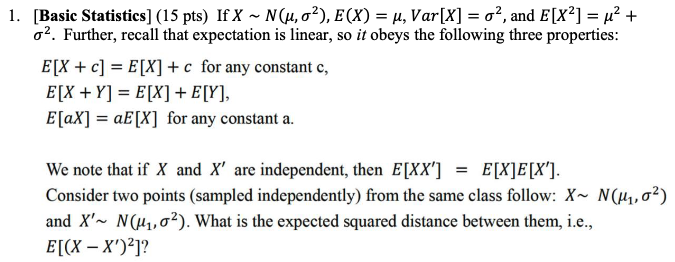
\includegraphics[width=1\textwidth]{media/hw2_q1.png}

\subsection{[Basic Linear Algebra] (15 pts) We are given a vector $x = [0, 0.2, 1.0, 2.2]$. Which of the following vector is closest to $x$ and what is the distance from the closest point to $x$ under each of the following vector norms?}

$$x_1 = [0.7, 0.2, 0.5, 2.0]$$
$$x_2 = [0, 1.0, 1.5, 2.2]$$
$$x_3 = [0.8, 0.1, 1.2, 2.0]$$

a) 0-norm =
b) 1-norm =
c) 2-norm =
d) $\infty$-norm =

\subsubsection{For $\mathbf{x_1}$:}
\begin{align}
    ||\mathbf{x} - \mathbf{x_1}|| &= 
    \begin{bmatrix}
        |0 - 0.7| & |0.2 - 0.2| & |1 - 0.5| & |2.2 - 2|
    \end{bmatrix} \nonumber \\
    &= 
    \begin{bmatrix}
        0.7 & 0 & 0.5 & 0.2
    \end{bmatrix} 
\end{align}
\begin{align}
    \Rightarrow ||\mathbf{x_1}||_0 &= 3
\end{align}
\begin{align}
    \Rightarrow  ||\mathbf{x_1}||_1 &= \sum ||\mathbf{x} - \mathbf{x_1}|| = 0.7 + 0 + 0.5 + 0.2 = 1.4
\end{align}
\begin{align}
    \Rightarrow ||\mathbf{x_1}||_2 &= \sqrt{|0 - 0.7|^2 + |0.2 - 0.2|^2 + |1 - 0.5|^2 + |2.2 - 2|^2} \nonumber \\
    &= \sqrt{0.7^2 + 0^2 + 0.5^2 + 0.2^2} = \sqrt{0.78} = 0.8832
\end{align}
\begin{align}
    \Rightarrow ||\mathbf{x_1}||_{\infty} &= max ||\mathbf{x} - \mathbf{x_1}|| = 0.7
\end{align}

\subsubsection{For $\mathbf{x_2}$:}
\begin{align}
    ||\mathbf{x} - \mathbf{x_2}|| &= 
    \begin{bmatrix}
        |0 - 0| & |0.2 - 1| & |1 - 1.5| & |2.2 - 2.2|
    \end{bmatrix} \nonumber \\
    &= 
    \begin{bmatrix}
        0 & 0.8 & 0.5 & 0
    \end{bmatrix} 
\end{align}
\begin{align}
    \Rightarrow ||\mathbf{x_2}||_0 &= 2
\end{align}
\begin{align}
    \Rightarrow  ||\mathbf{x_2}||_1 &= \sum ||\mathbf{x} - \mathbf{x_2}|| = 0 + 0.8 + 0.5 + 0 = 1.3
\end{align}
\begin{align}
    \Rightarrow ||\mathbf{x_2}||_2 &= \sqrt{|0 - 0|^2 + |0.2 - 1|^2 + |1 - 1.5|^2 + |2.2 - 2.2|^2} \nonumber \\
    &= \sqrt{0^2 + 0.8^2 + 0.5^2 + 0^2} = \sqrt{0.89} = 0.9434
\end{align}
\begin{align}
    \Rightarrow ||\mathbf{x_2}||_{\infty} &= max ||\mathbf{x} - \mathbf{x_2}|| = 0.8
\end{align}

\subsubsection{For $\mathbf{x_3}$:}
\begin{align}
    ||\mathbf{x} - \mathbf{x_3}|| &= 
    \begin{bmatrix}
        |0 - 0.8| & |0.2 - 0.1| & |1 - 1.2| & |2.2 - 2|
    \end{bmatrix} \nonumber \\
    &= 
    \begin{bmatrix}
        0.8 & 0.1 & 0.2 & 0.2
    \end{bmatrix} 
\end{align}
\begin{align}
    \Rightarrow ||\mathbf{x_3}||_0 &= 4
\end{align}
\begin{align}
    \Rightarrow  ||\mathbf{x_3}||_1 &= \sum ||\mathbf{x} - \mathbf{x_2}|| = 0.8 + 0.1 + 0.2 + 0.2 = 1.3
\end{align}
\begin{align}
    \Rightarrow ||\mathbf{x_3}||_2 &= \sqrt{|0 - 0.8|^2 + |0.2 - 0.1|^2 + |1 - 1.2|^2 + |2.2 - 2|^2} \nonumber \\
    &= \sqrt{0.8^2 + 0.1^2 + 0.2^2 + 0.2^2} = \sqrt{0.73} = 0.8544
\end{align}
\begin{align}
    \Rightarrow ||\mathbf{x_3}||_{\infty} &= max ||\mathbf{x} - \mathbf{x_3}|| = 0.8
\end{align}

Based on the above norm calculations, we have the following results:
\begin{enumerate}
    \item by the 0-norm, $\mathbf{x_2}$ is the closest to $\mathbf{x}$.
    \item by the 1-norm, both $\mathbf{x_2}$ and $\mathbf{x_3}$ are the closest to $\mathbf{x}$.
    \item by the 2-norm, $\mathbf{x_3}$ is the closest to $\mathbf{x}$.
    \item by the $\infty$-norm, $\mathbf{x_1}$ is the closest to $\mathbf{x}$.
\end{enumerate}

\subsection{[Convexity] (1)}

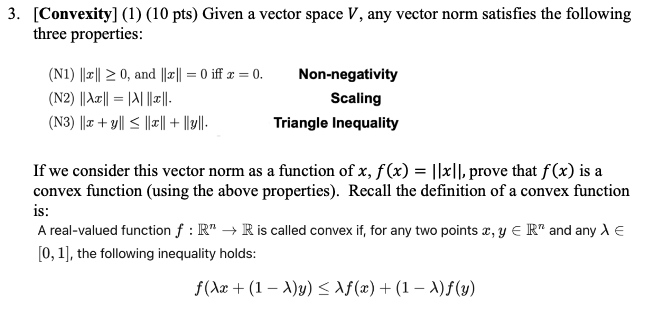
\includegraphics[width=1\textwidth]{media/hw2_q3.png}

\subsection{[Convexity] (2) (10 pts). Prove that the convexity is preserved under a linear transformation. Supposed $f(w)$ is convex in terms of $w$. Prove that $g(w)=f(X w + b)$ is also convex in terms of $w$ where $X$ is a fixed matrix of appropriate size, and $b$ is a fixed vector of appropriate size. (So $X$ and $b$ are not variables in $g$). (Hint: you can simply use the definition of convex function)}

\subsection{[Convexity] (3) (10 pts). From (1) and (2), prove the “loss” function $||y-Xw||_2$ is convex in terms of $w$ where $X_{n \times d}$ is a data matrix containing $n$ examples and each example has $d$ features, and $y$ is a column vector of length $d$. This dataset has been observed and thus fixed, and $w$ is the only variable in the norm.}  
\label{problems_end}

\end{document}
